\chapter{从伊辛磁体到液--气临界现象}

\lectureoverview{液--气转变可以通过一条出人意料的路径达到。我们首先完成对伊辛磁体的平均场处理，确定其共存线和临界点，然后把自旋向上重新解释为一个被占据的点阵位点。由此得到的点阵气体具有硬核排斥、短程吸引、由磁场控制的化学势，并且具有完全相同的相图。形式课程以临界行为和普适性作结。随后一个独立的课后讨论考察物理学家所说的精细调节是什么意思、选择效应如何可能进入一种解释，以及为什么这种推理只有与机制和可能的检验结合起来才有用。}

\section{为什么沸水始于一块磁体}

沸水是我们想要理解的熟悉现象：液体变成气体，其密度发生突变。标准路径经过范德瓦尔斯方程。这里我们走一条不同的路径。我们回到伊辛磁体，完成其平均场描述，然后发现同一个模型可以被读作一种流体。

这不仅仅是一个形象化的类比。一旦变量被正确地翻译，伊辛磁体和点阵气体就是同一个统计力学系统。磁化强度变成粒子密度，外磁场变成化学势，磁共存线变成液--气共存线。这一翻译解释了为什么两个表面上不同的物质部分可以具有相同的临界行为。

平均场在低维下不会给出精确的数值答案。在一维中，它甚至预言了一个精确解所禁止的转变。它在这里的价值是结构性的。在二维和三维中，它揭示了正确的序参量、相互竞争的相、临界端点，以及无穷小的偏置选择某一相的方式。在三维中，每个位点有六个最近邻，用它们的平均值代替这些近邻已经给出了有用的定性图像。

\section{伊辛能量的记账}

在超立方点阵的每个位点上放一个二态自旋，
\begin{equation}
\sigma_i=\pm1.
\end{equation}
我们使用哈密顿量
\begin{equation}
\mathcal H
=-J\sum_{\langle ij\rangle}\sigma_i\sigma_j
+h\sum_i\sigma_i,
\qquad J>0.
\label{eq:ising-hamiltonian}
\end{equation}
记号很重要。第一个求和是对最近邻\emph{连线}进行的；第二个求和是对\emph{位点}进行的。一条连线只被计数一次，而不是从每个端点各计数一次。

对于单条连线，
\begin{equation}
E_{ij}=-J\sigma_i\sigma_j.
\end{equation}
平行自旋具有能量\(-J\)，而反平行自旋具有能量\(+J\)。因此一个断键的代价是
\begin{equation}
\Delta E_{\rm bond}=+J-(-J)=2J.
\label{eq:broken-bond}
\end{equation}
控制相对玻尔兹曼权重的是\(2J\)这个数，而不是任何一个绝对的连线能量。我们可以给每个构型加上一个常数而不改变任何概率。

\begin{classroomqa}
\audiencequestion{为什么哈密顿量中有两个不同的求和？}
\lecturerresponse{交换能属于一对相邻位点，所以它是对连线\(\langle ij\rangle\)求和的。场独立地作用于每个自旋，所以它是对位点\(i\)求和的。混淆这两种计数方式恰好会引入那些在平均场中至关重要的因子二。\lecturetimestamp{00:08:04--00:08:45}}
\end{classroomqa}

\begin{classroomqa}
\audiencequestion{把\(J\)取得更大是否只是让每个能量都更负？}
\lecturerresponse{它增大了对齐构型与未对齐构型之间的间隔。能量的零点任意；物理陈述是，一个断键的代价是\(2J\)。因此，在固定温度下，更大的正\(J\)使热无序变得不那么有利。\lecturetimestamp{00:08:47--00:10:17}}
\end{classroomqa}

在\(d\)维的无限或周期性超立方点阵上，每个位点有\(2d\)个近邻。从所有\(N\)个位点计数会把每条连线计数两次，所以
\begin{equation}
N_{\rm links}=\frac{(2d)N}{2}=dN.
\label{eq:number-links}
\end{equation}
因此，一个对齐构型具有交换能\(-JdN\)。边界位点通过一个表面项改变这一点，在热力学极限下与\(N\)相比可以忽略。当\(h=0\)时，两个完全对齐的态是简并的。

场项固定了一个我们将始终一致保持的符号约定。在方程~\eqref{eq:ising-hamiltonian}中，正的\(h\)使\(\sigma=-1\)具有更低的位点能量。因此\(h>0\)有利于负磁化强度，而\(h<0\)有利于正磁化强度。人们可以通过写出\(-h\sum_i\sigma_i\)来反转这一约定；没有任何物理内容改变，但此后每个符号都必须随之反转。

\begin{classroomqa}
\audiencequestion{如果哈密顿量只包含\(J\)和\(h\)，温度从哪里进入？}
\lecturerresponse{温度通过玻尔兹曼因子\(e^{-\beta\mathcal H}\)进入，其中\(\beta=1/T\)，单位取\(k_{\rm B}=1\)。因此无量纲量是\(\beta J\)和\(\beta h\)。\lecturetimestamp{00:13:07--00:13:43}}
\end{classroomqa}

\section{一个自旋在其近邻的平均场中}

选取一个远离边界的自旋。它有\(2d\)个最近邻。平均场将每个涨落的近邻替换为同一个平均值
\begin{equation}
m=\expect{\sigma}.
\end{equation}
涉及所选自旋\(\sigma\)的交换能于是为
\begin{equation}
-J\sigma\sum_{\text{\(2d\) neighbors}}\sigma_j
\;\longrightarrow\;-2dJm\,\sigma.
\end{equation}
加上外场，得到有效的单自旋能量
\begin{equation}
\mathcal H_{\rm mf}(\sigma)=(-2dJm+h)\sigma.
\label{eq:mean-field-one-spin}
\end{equation}
因子\(2d\)是必不可少的。在写中心自旋图像时很容易漏掉它，而在板书推导中已明确将其恢复。

\begin{figure}[ht]
\centering
\includegraphics[width=0.84\textwidth]{lecture_10_figure_02.png}
\caption{一个中心自旋被其平均场近邻所包围，连同单自旋能量以及正在建立的自洽方程。}
\lectureframe{00:17:57}
\end{figure}

单自旋配分函数为
\begin{align}
z_{\rm mf}
&=\sum_{\sigma=\pm1}
\exp\!\left[-\beta(-2dJm+h)\sigma\right] \\
&=2\cosh\!\left[\beta(2dJm-h)\right].
\end{align}
其平均自旋为
\begin{align}
\expect{\sigma}
&=\frac{\sum_{\sigma=\pm1}\sigma
 e^{\beta(2dJm-h)\sigma}}
{\sum_{\sigma=\pm1}e^{\beta(2dJm-h)\sigma}} \\
&=\tanh\!\left[\beta(2dJm-h)\right].
\end{align}
但我们所选的自旋应当代表那些其平均值被我们记作\(m\)的近邻。因此自洽性要求
\begin{equation}
\boxed{m=\tanh\!\left[\beta(2dJm-h)\right].}
\label{eq:mean-field-self-consistency}
\end{equation}
这一个非线性方程就是多自旋问题的平均场约化。

\begin{classroomqa}
\audiencequestion{为什么左边的平均值与为每个近邻代入的\(m\)相同？}
\lecturerresponse{这个等式就是近似。我们假定一个均匀的体态，将实际环境替换为其平均值，在该环境中计算中心自旋，并要求计算出的平均值再现我们所假定的环境。一个解就是一个自洽的体态。\lecturetimestamp{00:16:28--00:18:00}}
\end{classroomqa}

引入
\begin{equation}
y=2\beta dJm.
\label{eq:y-definition}
\end{equation}
由于\(\beta=1/T\)，
\begin{equation}
m=\frac{yT}{2dJ},
\end{equation}
而方程~\eqref{eq:mean-field-self-consistency}变为
\begin{equation}
\boxed{\frac{yT}{2dJ}=\tanh(y-\beta h).}
\label{eq:reduced-mean-field}
\end{equation}

\begin{figure}[ht]
\centering
\includegraphics[width=0.82\textwidth]{lecture_10_figure_03.png}
\caption{引入\(y=2\beta dJm\)后的约化自洽方程，已准备好用图解法求解。}
\lectureframe{00:24:42}
\end{figure}

\begin{classroomqa}
\audiencequestion{为什么场以\(y-\beta h\)的形式出现，而正场偏向哪个自旋？}
\lecturerresponse{我们的哈密顿量包含\(+h\sigma\)。因此其玻尔兹曼指数为\(\beta(2dJm-h)\sigma\)，所以双曲正切中包含\(y-\beta h\)。正的\(h\)偏向\(\sigma=-1\)。如果改用\(-h\sigma\)来定义哈密顿量，则\(h\)的每一次出现都改变符号，相图被水平反射。\lecturetimestamp{00:18:17--00:20:00}}
\end{classroomqa}

\section{图解解与居里点}

令\(h=0\)。我们必须求出
\begin{equation}
\frac{T}{2dJ}y
\qquad\text{and}\qquad
\tanh y.
\end{equation}
的交点。第一条是过原点的直线；第二条是奇函数、饱和的曲线。在高温下直线很陡，唯一的交点是\(y=0\)，因此\(m=0\)。随着温度下降，直线变得较平缓。当直线与双曲正切在原点相切时，达到临界温度。

\begin{figure}[ht]
\centering
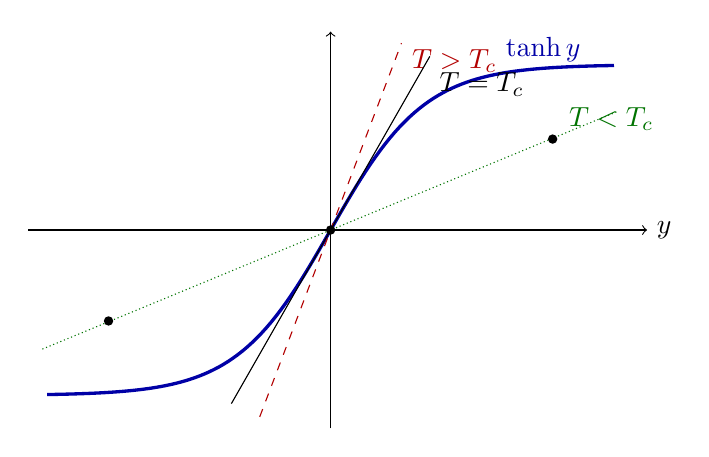
\begin{tikzpicture}[x=1.2cm,y=2.1cm]
\draw[->] (-3.2,0) -- (3.35,0) node[right] {$y$};
\draw[->] (0,-1.2) -- (0,1.2);
\draw[very thick,blue!65!black,domain=-3:3,samples=120]
  plot (\x,{tanh(\x)});
\node[blue!65!black,above] at (2.25,0.96) {$\tanh y$};
\draw[dashed,red!70!black] (-0.75,-1.13) -- (0.75,1.13);
\node[red!70!black,right] at (0.76,1.02) {$T>T_c$};
\draw[black] (-1.05,-1.05) -- (1.05,1.05);
\node[right] at (1.05,0.88) {$T=T_c$};
\draw[densely dotted,green!45!black] (-3.05,-0.72) -- (3.05,0.72);
\node[green!45!black,right] at (2.42,0.67) {$T<T_c$};
\fill (-2.35,-0.55) circle (1.7pt);
\fill (0,0) circle (1.7pt);
\fill (2.35,0.55) circle (1.7pt);
\end{tikzpicture}
\caption{零场下的平均场方程。在\(T_c\)以下，两个非零交点代表稳定的磁化相；零解在代数上仍然存在，但已不稳定。}
\label{fig:mean-field-intersections}
\end{figure}

因为
\begin{equation}
\left.\frac{d}{dy}\tanh y\right|_{y=0}=1,
\end{equation}
所以相切条件为
\begin{equation}
\frac{T_c}{2dJ}=1.
\end{equation}
因此平均场预言
\begin{equation}
\boxed{T_c^{\rm MF}=2dJ.}
\label{eq:sm10-mean-field-tc}
\end{equation}
在此温度以下有两个稳定的非零解\(\pm m_0(T)\)。解\(m=0\)仍然满足方程，但它不再是稳定平衡。系统选择两个对称相关的磁化相之一。

\begin{classroomqa}
\audiencequestion{这就是居里温度吗？}
\lecturerresponse{是的。对于铁磁体，自发磁化消失的温度按惯例称为居里温度。这里\(2dJ\)是它的平均场值，而不是精确的低维结果。\lecturetimestamp{00:28:19--00:28:57}}
\end{classroomqa}

在转变附近，展开双曲正切：
\begin{equation}
\tanh y=y-\frac{y^3}{3}+O(y^5).
\end{equation}
在\(h=0\)处，方程~\eqref{eq:reduced-mean-field}给出
\begin{equation}
\left(1-\frac{T}{T_c}\right)y-\frac{y^3}{3}+O(y^5)=0.
\end{equation}
因此非零分支的行为为
\begin{equation}
y^2\simeq3\left(1-\frac{T}{T_c}\right),
\qquad
m\propto(T_c-T)^{1/2}.
\label{eq:mf-beta-exponent}
\end{equation}
这个平方根是一个平均场临界指数。其精确值在低维下将不再成立，但序参量在端点处连续消失这一点将会保留。

\section{温度--场平面与分支选择}

材料固定\(J\)；实验者可以改变\(T\)和\(h\)。因此自然要在\(T\)--\(h\)平面中画出相图。在\(T_c\)以下，任意小的场都会选择两个磁化分支之一。按照我们的约定，\(h<0\)选择\(m>0\)，而\(h>0\)选择\(m<0\)。

在零温下，自旋完全排列整齐，因此 \(m=\pm1\)。在高温下，零场平均值为 \(m=0\)。当沿 \(h=0\) 趋近临界点时，量值 \(m_0(T)\) 连续地降为零。但在任意固定的 \(T<T_c\) 下，穿过 \(h=0\) 时，会从 \(+m_0(T)\) 不连续地切换到 \(-m_0(T)\)。

\begin{figure}[ht]
\centering
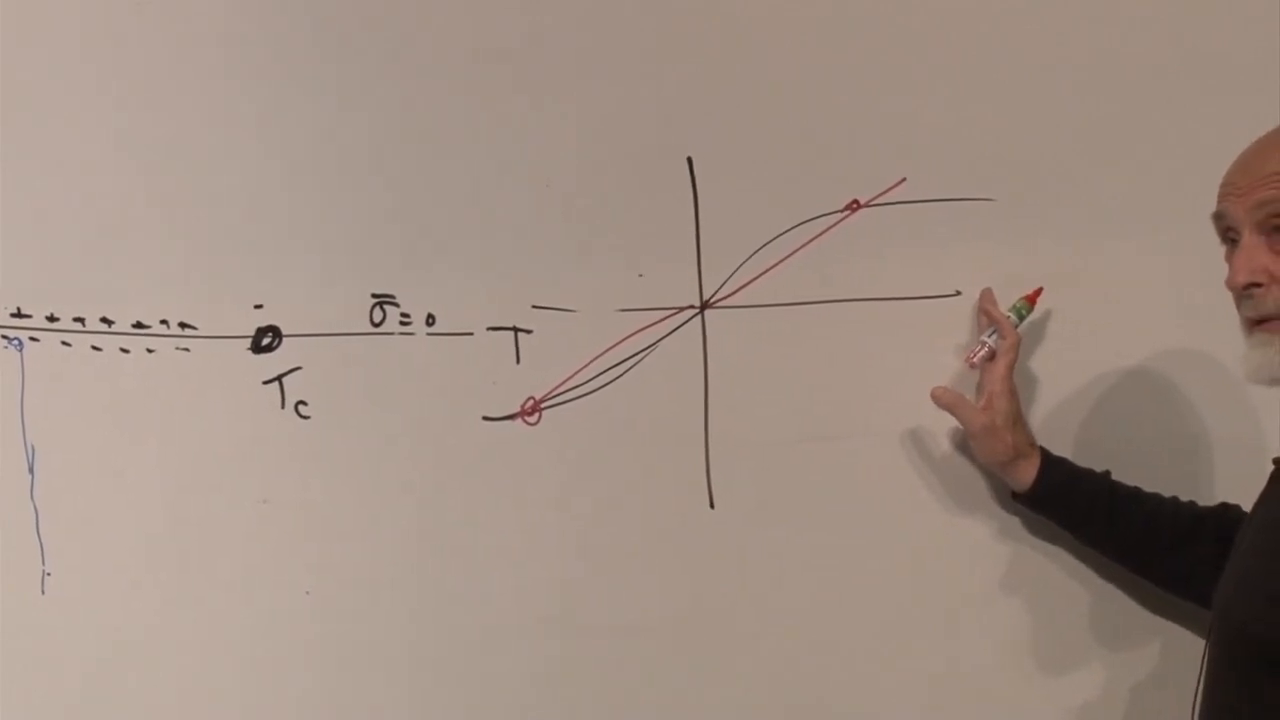
\includegraphics[width=0.90\textwidth]{lecture_10_figure_06.png}
\caption{\(T\)--\(h\) 平面中的共存线，以及温度低于 \(T_c\) 时固定温度下的磁化强度分支。}
\lectureframe{00:39:30}
\end{figure}

\begin{figure}[ht]
\centering
\resizebox{\linewidth}{!}{%
\begin{tikzpicture}[x=1.25cm,y=1.15cm]
\begin{scope}
\draw[->] (-2.45,0) -- (2.55,0) node[right] {$h$};
\draw[->] (0,0) -- (0,3.7) node[above] {$T$};
\draw[very thick,red!70!black] (0,0) -- (0,2.35);
\fill[red!70!black] (0,2.35) circle (2.3pt);
\node[right] at (0.08,2.35) {$T_c$};
\node at (-1.25,1.05) {$m>0$};
\node at (1.25,1.05) {$m<0$};
\draw[->,rounded corners,blue!65!black] (-1.65,0.85) -- (-1.65,3.02)
 -- (1.65,3.02) -- (1.65,0.85);
\node[blue!65!black] at (0,3.35) {continuous path};
\end{scope}
\begin{scope}[xshift=7.0cm,yshift=1.55cm]
\draw[->] (-2.5,0) -- (2.5,0) node[right] {$h$};
\draw[->] (0,-1.35) -- (0,1.4) node[above] {$m$};
\draw[very thick,blue!65!black]
  (-2.2,1.05) .. controls (-0.75,1.03) and (-0.2,0.75) .. (-0.08,0.62);
\draw[very thick,blue!65!black]
  (0.08,-0.62) .. controls (0.2,-0.75) and (0.75,-1.03) .. (2.2,-1.05);
\draw[dashed] (0,0.62) -- (0,-0.62);
\fill (0,0.62) circle (1.8pt);
\fill (0,-0.62) circle (1.8pt);
\node at (0,-1.75) {\(T<T_c\)};
\end{scope}
\end{tikzpicture}
}
\caption{在固定的 \(T<T_c\) 下，磁化强度在穿过共存线时发生跳变。而在完整的两参数平面中，两个相反而可以通过绕过临界点的方式连续地连接起来。}
\label{fig:ising-phase-plane}
\end{figure}

\begin{classroomqa}
\audiencequestion{如果在 \(T_c\) 以下磁场恰好为零，会发生什么？}
\lecturerresponse{理想的无限系统有两个同样好的纯相。任何与制备相关的无穷小残余偏置、边界条件或涨落都会选择其中之一。热力学不连续性由我们的符号约定中的两个单侧极限 \(m(T,0^-)=+m_0(T)\) 和 \(m(T,0^+)=-m_0(T)\) 来表示。\lecturetimestamp{00:35:04--00:37:10}}
\end{classroomqa}

\begin{classroomqa}
\audiencequestion{这和滞后是同一回事吗？}
\lecturerresponse{滞后涉及亚稳性以及真实系统切换分支时所表现出的依赖于历史的延迟。它与上述问题相关，但需要超出平衡相图的动力学，此处不予展开。\lecturetimestamp{00:37:11--00:37:20}}
\end{classroomqa}

\begin{classroomqa}
\audiencequestion{正相和负相能否在不穿过不连续点的情况下连接起来？}
\lecturerresponse{可以。将温度升高到 \(T_c\) 以上，在那里改变磁场的符号，然后再降低温度。这条路径绕过了端点，磁化强度连续地变化。只有当在固定的 \(T<T_c\) 下穿过 \(h=0\) 时，跳变才是不可避免的。\lecturetimestamp{00:37:20--00:38:15}}
\end{classroomqa}

\begin{classroomqa}
\audiencequestion{每当 \(h\) 趋近于零时，磁化强度都会趋近于零吗？}
\lecturerresponse{在 \(T_c\) 以下的一般温度下并非如此。在那里，单侧极限不为零。自发磁化强度只有在临界温度本身被趋近时才会趋近于零。\lecturetimestamp{00:38:29--00:39:45}}
\end{classroomqa}

\section{可渗透盒子与化学势}

现在我们离开磁体，重新从粒子开始。设想一个区域，其势能低于周围空间的势能。壁是可渗透的：粒子可以进入和离开。如果内部能量低了 \(\mu\)，那么内部占据会获得一个相对的玻尔兹曼因子 \(e^{\beta\mu}\)。加深或抬高势阱会改变盒子中粒子的平均数目。

\begin{figure}[ht]
\centering
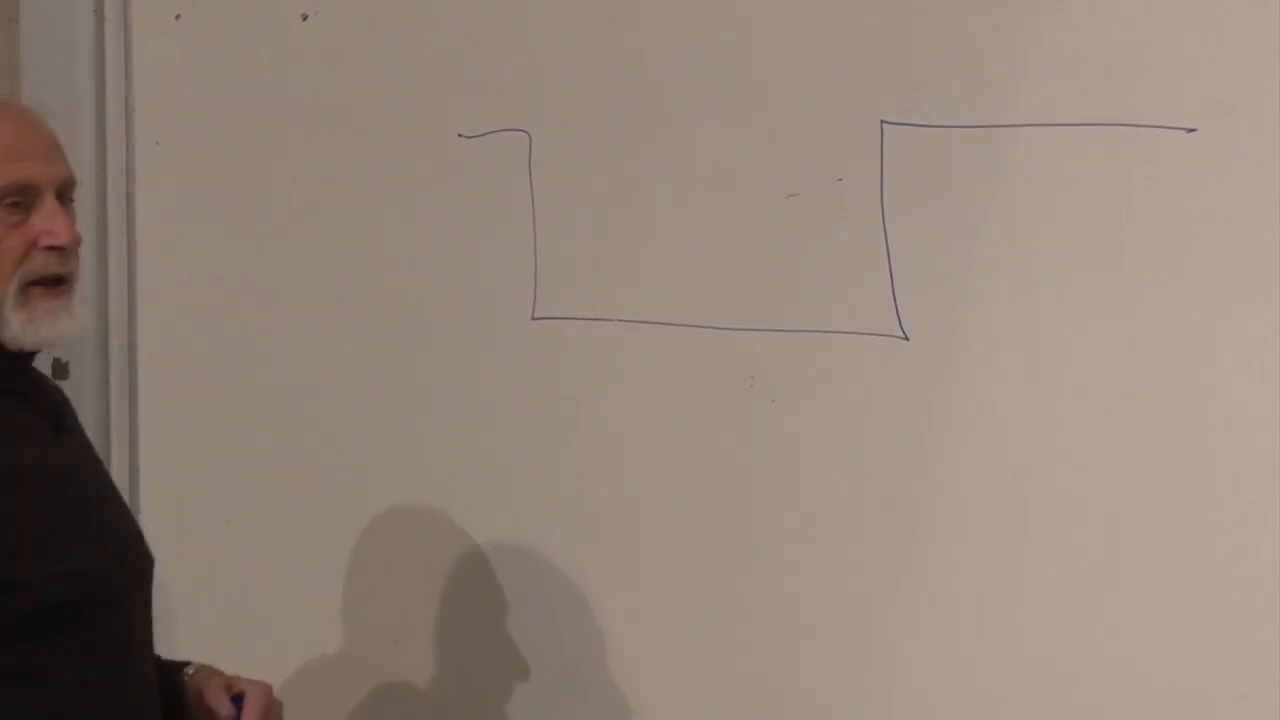
\includegraphics[width=0.84\textwidth]{lecture_10_figure_07.png}
\caption{可渗透盒子的势阱图像。内部与外部之间的能量差控制着粒子占据盒子的倾向。}
\lectureframe{00:41:30}
\end{figure}

\begin{figure}[ht]
\centering
\resizebox{\linewidth}{!}{%
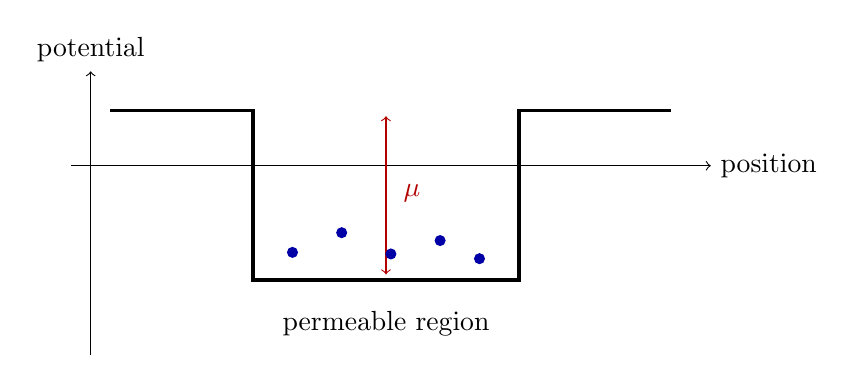
\begin{tikzpicture}[x=1.25cm,y=1.0cm]
\draw[->] (-3.2,0) -- (3.3,0) node[right] {position};
\draw[->] (-3.0,-2.4) -- (-3.0,1.2) node[above] {potential};
\draw[very thick] (-2.8,0.7) -- (-1.35,0.7)
 -- (-1.35,-1.45) -- (1.35,-1.45) -- (1.35,0.7) -- (2.9,0.7);
\draw[<->,red!70!black] (0,0.63) -- (0,-1.38);
\node[right,red!70!black] at (0.08,-0.35) {$\mu$};
\foreach \x/\y in {-0.95/-1.1,-0.45/-0.85,0.05/-1.12,0.55/-0.95,0.95/-1.18}
  \fill[blue!65!black] (\x,\y) circle (2pt);
\node at (0,-2.0) {permeable region};
\end{tikzpicture}
}
\caption{改变势偏移会改变粒子数偏好。在巨正则描述中，该偏移由化学势表示。}
\end{figure}

这个思想实验使化学势变得具体。它是相对于粒子库而言，每增加一个粒子所获得的能量优势。如果多种粒子种类能够穿过壁，那么每种粒子种类都有自己的化学势。密封盒子则不同：此时 \(N\) 是固定的，化学势是通过热力学推断出来的，而不是通过与粒子库的交换来施加的。

\begin{classroomqa}
\audiencequestion{势阱的深度就是化学势吗？}
\lecturerresponse{它是化学势差的一种直接力学实现。将内部每一个单粒子能级降低 \(\mu\)，会对能量贡献 \(-\mu N\)，因此对玻尔兹曼指数贡献 \(+\beta\mu N\)。只有化学势的差值才有意义。\lecturetimestamp{00:44:49--00:45:40}}
\end{classroomqa}

由于粒子可以进入和离开，配分和必须包含所有粒子数：
\begin{equation}
\Xi(T,\mu)
=\sum_{N=0}^{\infty}\;\sum_{\mathcal C_N}
\exp\!\left[-\beta E(\mathcal C_N)+\beta\mu N\right].
\label{eq:grand-partition}
\end{equation}
内层求和遍历具有指定 \(N\) 的构型；外层求和遍历 \(N\) 本身。巨正则权重也可以写成 \(e^{-\beta(E-\mu N)}\)。

\begin{figure}[ht]
\centering
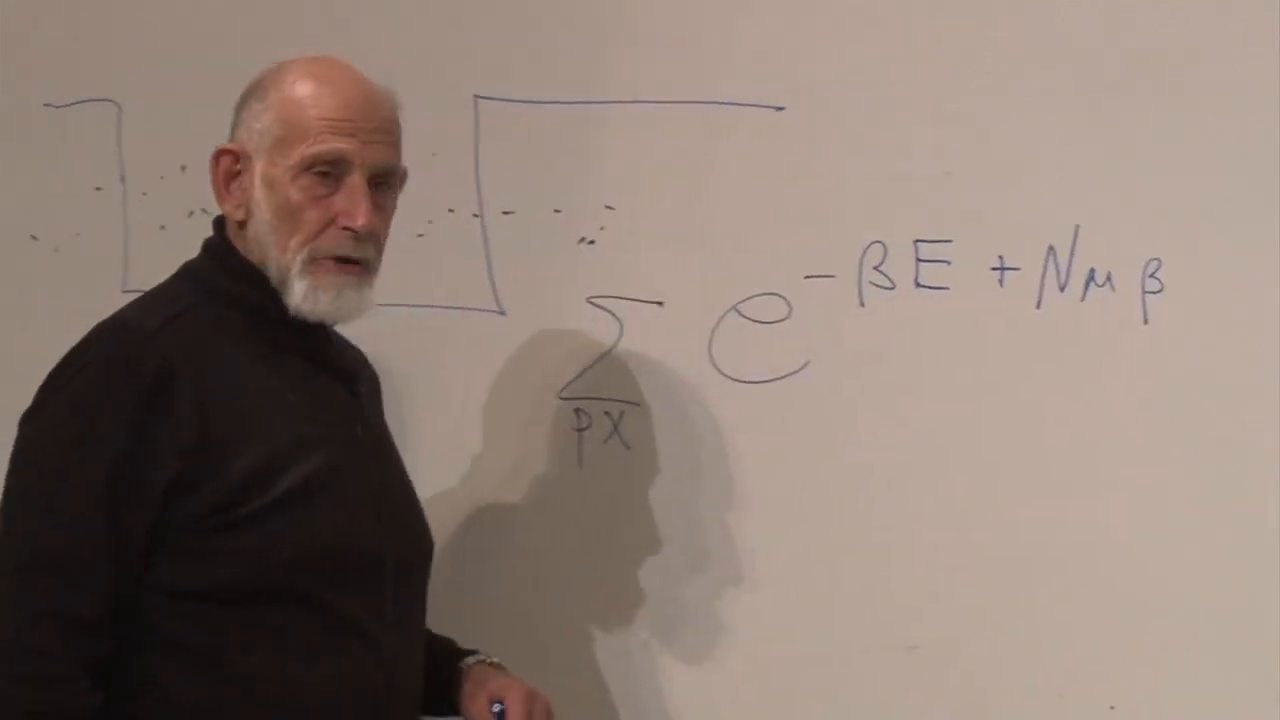
\includegraphics[width=0.88\textwidth]{lecture_10_figure_08.png}
\caption{可渗透盒子以及对粒子数和构型的巨正则求和。}
\lectureframe{00:47:15}
\end{figure}

\begin{classroomqa}
\audiencequestion{当盒子被密封时，会有什么变化？}
\lecturerresponse{粒子数不再涨落。此时使用固定 \(N\) 下的正则配分函数。在可渗透盒子中，\(N\) 是一个热力学变量，其平均值由 \(\mu\) 控制。\lecturetimestamp{00:45:42--00:47:50}}
\end{classroomqa}

在固定温度下，改变 \(\mu\) 通常会使密度平滑变化。低于临界温度时，它反而可能引起突变。这正是我们要寻找的流体现象。为了从微观上得到它，粒子需要两个特征：它们不能占据同一位置，并且必须在短程上相互吸引。

\section{将自旋转化为点阵气体}

保留点阵，但重新解释它的两个状态。定义占据数
\begin{equation}
n_i=\frac{1+\sigma_i}{2}
=
\begin{cases}
0,&\sigma_i=-1,\\
1,&\sigma_i=+1.
\end{cases}
\label{eq:occupation-map}
\end{equation}
空位点具有自旋向下；被占据的位点具有自旋向上。由于 \(n_i\) 只能为零或一，双重占据被禁止。因此点阵本身提供了硬核。

\begin{figure}[ht]
\centering
\includegraphics[width=0.84\textwidth]{lecture_10_figure_04.png}
\caption{点阵气体的对应从 \(\sigma=-1\) 表示空位点开始；\(\sigma=+1\) 则表示被占据的位点。}
\lectureframe{00:53:45}
\end{figure}

从空点阵开始，所有 \(\sigma=-1\)。每条键都对齐，能量为 \(-J\)。这个恒定的真空能量可以被减去。现在在二维中把一个粒子放在一个位点上。相应的自旋翻转到 \(+1\)，破坏了四条键。每条被破坏的键代价为 \(2J\)，所以
\begin{equation}
\Delta E_1=4(2J)=8J.
\label{eq:one-particle-cost}
\end{equation}
两个相距很远的粒子破坏八条键，代价为 \(16J\)。如果这两个粒子占据相邻位点，它们之间的键重新对齐。只有六条边界键被破坏，代价为
\begin{equation}
\Delta E_{2,\rm adjacent}=6(2J)=12J.
\end{equation}
因此，把粒子拉到一起会使能量降低
\begin{equation}
16J-12J=4J.
\label{eq:lattice-attraction}
\end{equation}
这个实时计数最初被描述为 \(2J\) 的节省，随后得到更正：一条共享的键消除了两个被破坏边界的贡献，因此吸引为 \(4J\)。

\begin{figure}[ht]
\centering
\includegraphics[width=0.84\textwidth]{lecture_10_figure_05.png}
\caption{二维键计数：一个孤立粒子代价为 \(8J\)，两个远离的粒子代价为 \(16J\)，两个相邻粒子代价为 \(12J\)。}
\lectureframe{01:00:25}
\end{figure}

点阵气体现在具有两个所需的分子性质。二元占据提供了硬核排斥，交换相互作用提供了强度为 \(4J\) 的最近邻吸引。粒子数被允许涨落，因为自旋翻转会改变被占据位点的数目。

\subsection{精确的代数对应词典}

键计数图像足以看出物理，但精确的变量替换使等价性无可置疑。将
\begin{equation}
\sigma_i=2n_i-1
\end{equation}
代入方程 ~\eqref{eq:ising-hamiltonian}。对于一条键，
\begin{equation}
\sigma_i\sigma_j
=4n_in_j-2n_i-2n_j+1.
\end{equation}
在规则的 \(d\) 维点阵上，
\begin{equation}
\sum_{\langle ij\rangle}(n_i+n_j)=2d\sum_i n_i.
\end{equation}
因此
\begin{align}
\mathcal H
&=-4J\sum_{\langle ij\rangle}n_in_j
+(4dJ+2h)\sum_i n_i+\text{constant}.
\label{eq:ising-as-lattice-gas}
\end{align}
将其与常规的点阵气体哈密顿量
\begin{equation}
\mathcal H_{\rm lg}
=-\epsilon\sum_{\langle ij\rangle}n_in_j
-\mu\sum_i n_i+\text{constant}.
\label{eq:lattice-gas-hamiltonian}
\end{equation}
比较。对应词典为
\begin{equation}
\boxed{\epsilon=4J,\qquad
\mu=-(4dJ+2h).}
\label{eq:chemical-potential-map}
\end{equation}

\begin{figure}[ht]
\centering
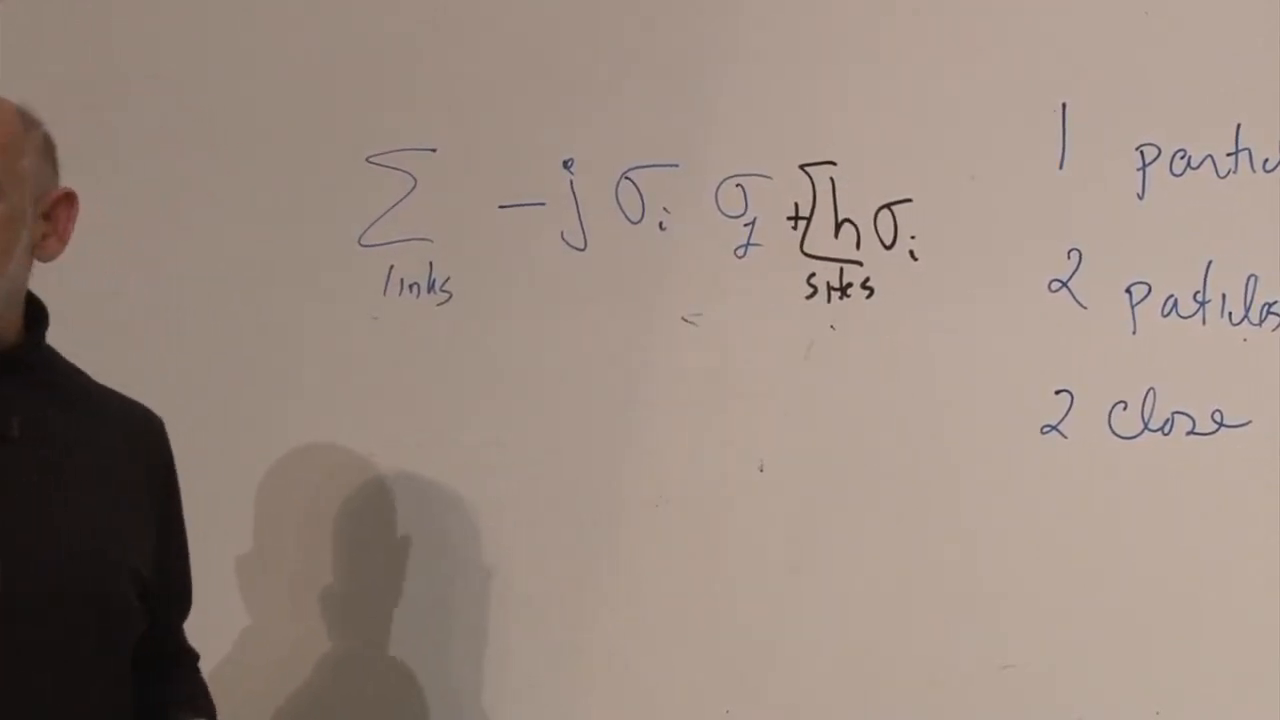
\includegraphics[width=0.88\textwidth]{lecture_10_figure_09.png}
\caption{交换项和场项与粒子能量计数并列。场改变插入能量，而不改变最近邻吸引。}
\lectureframe{01:04:30}
\end{figure}

在二维中，一次孤立插入使能量改变
\begin{equation}
8J+2h=-\mu.
\end{equation}
\(8J\) 来自被破坏的键；\(2h\) 来自将一个自旋从 \(-1\) 变为 \(+1\)。因此，调节 \(h\) 会调节化学势，同时保持吸引 \(4J\) 固定。场并不字面等于 \(\mu\)，因为交换基线贡献了偏移 \(4dJ\)。

\begin{classroomqa}
\audiencequestion{如果场控制粒子数，为什么 \(h\) 不简单地就是化学势？}
\lecturerresponse{创建一个粒子相对于空参考态也会破坏交换键。因此 \(-N\) 的常规系数是 \(\mu=-(4dJ+2h)\)，而不仅仅是 \(-2h\)。该偏移取决于 \(J\) 和配位数。\lecturetimestamp{01:06:28--01:06:41}}
\end{classroomqa}

密度同样简单：
\begin{equation}
\rho=\expect{n_i}
=\frac{1+\expect{\sigma_i}}{2}
=\frac{1+m}{2}.
\label{eq:density-map}
\end{equation}
因此 \(m=-1\) 是空点阵，\(m=+1\) 是完全填满的点阵，而 \(m=0\) 是半填充。总粒子数为 \(N_{\rm p}=\sum_i n_i\)；密度为 \(N_{\rm p}/N\)。

\begin{figure}[ht]
\centering
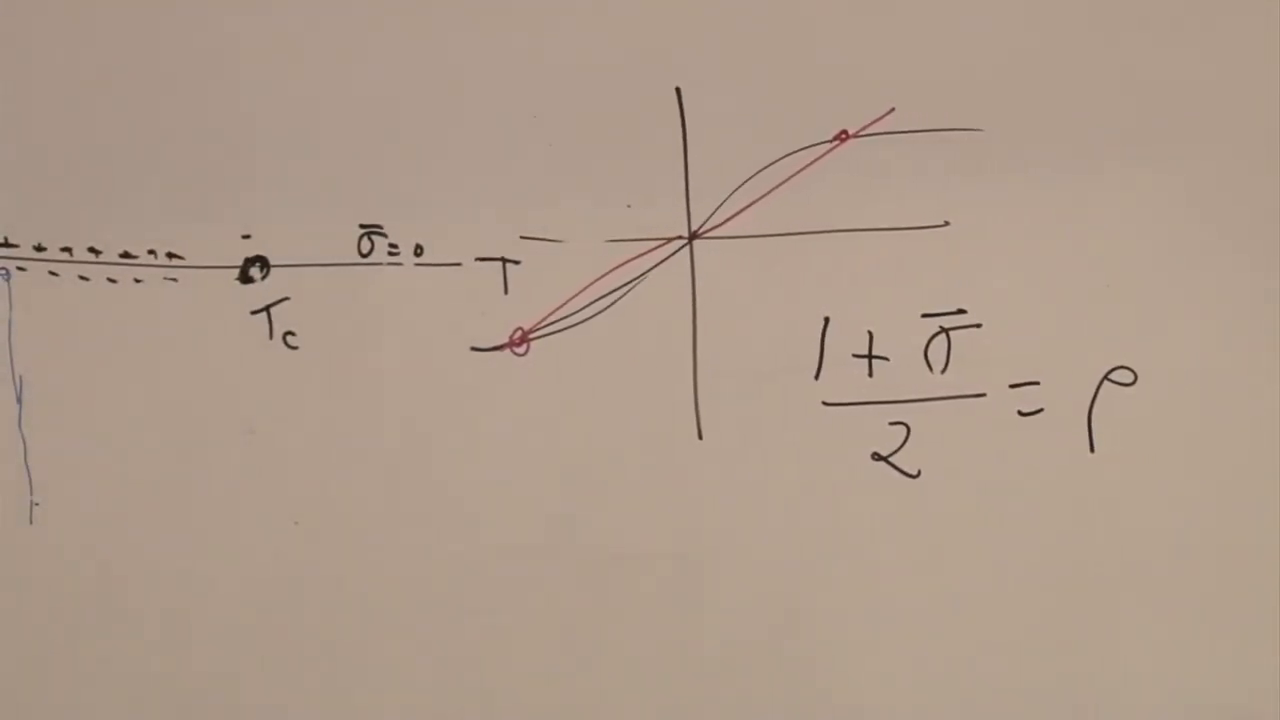
\includegraphics[width=0.90\textwidth]{lecture_10_figure_10.png}
\caption{密度关系 \(\rho=(1+m)/2\) 写在磁共存线旁边。}
\lectureframe{01:08:25}
\end{figure}

\begin{classroomqa}
\audiencequestion{\((1+m)/2\) 是粒子数还是密度？}
\lecturerresponse{它是每个位点的平均占据数，因此是无量纲的点阵密度。乘以总位点数就得到预期的粒子数。区分强度量密度和广延量计数很重要。\lecturetimestamp{01:06:43--01:09:31}}
\end{classroomqa}

\section{磁相图变为流体相图}

利用方程 ~\eqref{eq:chemical-potential-map} 和 \eqref{eq:density-map} 翻译图 ~\ref{fig:ising-phase-plane}。在 \(T_c\) 以上，改变 \(\mu\) 会平滑地改变密度。在 \(T_c\) 以下，越过共存值
\begin{equation}
\mu_{\rm coex}=-4dJ
\qquad(h=0)
\label{eq:coexistence-mu}
\end{equation}
会使密度在稀薄气体和稠密液体之间跳跃。在 \(T_c\) 处，两个密度合并，不连续性消失。

\begin{figure}[ht]
\centering
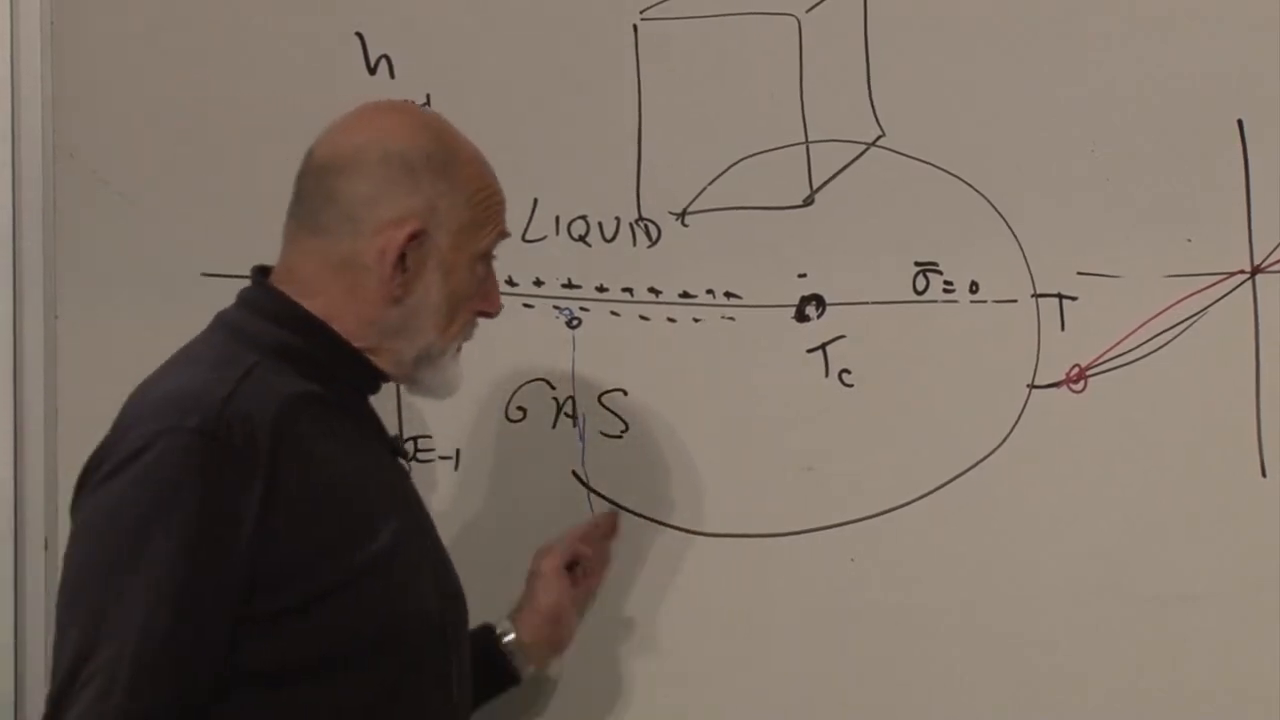
\includegraphics[width=0.92\textwidth]{lecture_10_figure_11.png}
\caption{伊辛共存线被解读为液--气相图。气体位于低密度一侧，液体位于高密度一侧，二者可以绕过临界端点连续地连接起来。}
\lectureframe{01:14:30}
\end{figure}

\begin{figure}[ht]
\centering
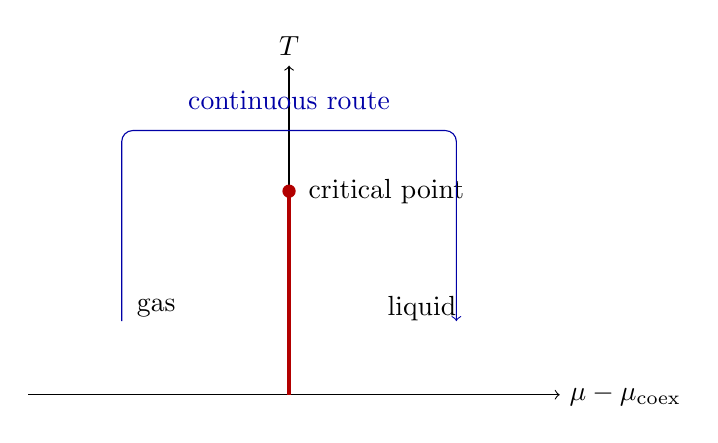
\begin{tikzpicture}[x=1.25cm,y=1.1cm]
\draw[->] (-2.65,0) -- (2.75,0) node[right] {$\mu-\mu_{\rm coex}$};
\draw[->] (0,0) -- (0,3.8) node[above] {$T$};
\draw[very thick,red!70!black] (0,0) -- (0,2.35);
\fill[red!70!black] (0,2.35) circle (2.4pt);
\node[right] at (0.1,2.35) {critical point};
\node at (-1.35,1.0) {gas};
\node at (1.35,1.0) {liquid};
\draw[->,blue!65!black,rounded corners]
 (-1.7,0.85) -- (-1.7,3.05) -- (1.7,3.05) -- (1.7,0.85);
\node[blue!65!black] at (0,3.4) {continuous route};
\end{tikzpicture}
\caption{在端点以下，液体和气体是彼此不同的相，但在超临界区域，并没有奇异的边界将它们分开。}
\label{fig:liquid-gas-plane}
\end{figure}

这就识别出了我们所熟悉的沸腾线。在固定压强下，将液体加热至越过共存线便产生沸腾。在固定温度下，改变压强或化学势也可以越过同一条边界。过热蒸气或过冷液体是超出平衡共存线的亚稳态延续；描述其寿命需要成核动力学，这超出了本平衡态构造的范围。

\begin{classroomqa}
\audiencequestion{过热蒸汽在这个相图中有所体现吗？}
\lecturerresponse{平衡相图标示的是共存边界。过热或过饱和状态是亚稳态的：它暂时停留在错误的一侧，因为形成临界液滴需要付出界面自由能的代价。这种动力学上的修正此处不予计算。 \lecturetimestamp{01:12:19--01:12:29}}
\end{classroomqa}

\begin{classroomqa}
\audiencequestion{在普通流体中，人们如何改变化学势？}
\lecturerresponse{势阱盒子是干净的理论控制手段。在实验室中，人们更常改变压强、体积或与热库的接触；热力学随后会将这些控制量转化为化学势的变化。 \lecturetimestamp{01:12:30--01:13:59}}
\end{classroomqa}

\begin{classroomqa}
\audiencequestion{当密度改变时，我们是在改变分子势 \(J\) 吗？}
\lecturerresponse{不是。对于固定的一种物质，\(J\) 代表短程吸引，并且在这个模型中保持不变。改变 \(\mu\) 会改变有多少格点被占据，从而改变分子间间距的分布。改变 \(J\) 则意味着改变微观物质或相互作用。 \lecturetimestamp{01:14:50--01:15:41}}
\end{classroomqa}

\begin{classroomqa}
\audiencequestion{临界温度和通常所说的沸点是同一回事吗？}
\lecturerresponse{不是。沸点是在选定的压强下确定的，因此当压强改变时，它沿共存曲线移动。临界温度是唯一的端点，高于它液体和气体不再被相边界分开。在这个点阵气体处理中，压强尚未被显式地推导出来。 \lecturetimestamp{01:15:42--01:17:02}}
\end{classroomqa}

现在可以陈述核心结果了。伊辛磁体与点阵气体并不只是画出相似的相图。在变量和参数变换之后，它们共享同一个配分函数。一侧的每一个奇异热力学性质在另一侧都有对应物：
\begin{equation}
\begin{array}{c|c}
\text{Ising magnet} & \text{lattice gas}\\ \hline
\sigma_i=\pm1 & n_i=0,1\\
m=\expect{\sigma} & \rho=(1+m)/2\\
h & \mu=-(4dJ+2h)\\
\text{aligned exchange} & \text{nearest-neighbor attraction}\\
h=0,\ T<T_c & \text{liquid--gas coexistence}\\
(T_c,0) & \text{critical endpoint}
\end{array}
\label{eq:ising-fluid-dictionary}
\end{equation}

\section{临界指数与普适性}

在临界点附近，热力学量常常出现幂律奇异性。以约化温度
\begin{equation}
t=\frac{T-T_c}{T_c},
\end{equation}
可示意性地写出
\begin{equation}
m\sim(-t)^{\beta_{\rm crit}},
\qquad
\chi\sim |t|^{-\gamma},
\qquad
\xi\sim |t|^{-\nu}.
\label{eq:critical-exponents}
\end{equation}
这里 \(\beta_{\rm crit}\) 是临界指数，而不是温度的倒数。平均场给出 \(\beta_{\rm crit}=1/2\)，但在上临界维度以下，涨落会改变这些指数。

这些指数不必是整数。它们也不必都是无理数：二维伊辛模型以拥有若干精确的有理指数而闻名，而三维伊辛模型的指数则是通过理论和计算以高精度确定下来的非平凡数值。稳健的教训是，这些指数一般并不由初等的量纲分析所固定。

更引人注目的是，微观细节往往也不能固定它们。具有相同空间维度、相同序参量对称性以及足够短程相互作用的系统，可以流向同一个长距离临界理论。它们属于同一个 \emph{普适类}。单轴磁体和普通液--气端点都具有单个标量序参量，并在相同维度下共享伊辛普适类。

\begin{classroomqa}
\audiencequestion{普适类是有限的还是离散的清单？}
\lecturerresponse{普适类有很多，按维度、对称性、守恒律、相互作用程以及其他长距离数据来组织。在许多熟悉的情形中，不动点和指数集合是离散的，但也存在指数连续变化的系统。稳妥的说法并不是这个目录是有限的；而是许多微观上不同的系统共享相同的长距离数据。 \lecturetimestamp{01:18:50--01:19:38}}
\end{classroomqa}

\begin{classroomqa}
\audiencequestion{如果液体和气体共存，在实际容器中是什么把它们分开？}
\lecturerresponse{是界面。表面张力对界面面积施加惩罚，而重力产生竖直的化学势梯度，通常使较密的液体位于气体下方。在重力可忽略时，几何形状更直接地由表面张力和边界条件控制。\lecturetimestamp{01:19:40--01:21:18}}
\end{classroomqa}

\begin{classroomqa}
\audiencequestion{在这幅图像中，汽化热在哪里？}
\lecturerresponse{在临界点以下，穿过一阶共存线通常会伴随潜热。当接近临界端点时，汽化热趋于零，因为两相在那里变得相同。本讲建立了相结构，但没有计算潜热。\lecturetimestamp{01:21:19--01:22:18}}
\end{classroomqa}

\begin{classroomqa}
\audiencequestion{相变能否用作灵敏探测器，例如用超导器件？}
\lecturerresponse{可以。在相变附近，微小的扰动可以产生很大的响应，或触发状态改变。实用探测器正是利用这种灵敏度，尽管相关的序参量和动力学可能与伊辛例子不同。\lecturetimestamp{01:22:19--01:24:05}}
\end{classroomqa}

统计力学课程到此结束。这条路线从熵和平衡开始，经过配分函数和气体，最后表明磁体和流体可以是同一临界现象的两种描述。

\section{课后讨论：精细调节与选择}

正式讲座结束后，谈话又持续了大约四十分钟。它值得保留，但不应与上面的推导相混淆。主题不再是点阵气体，而是精细调节的逻辑以及宇宙学中人类选择原理的谨慎使用。

\subsection{小数字并不自动意味着精细调节}

没有任何一句话能解决\emph{人类原理}这一短语的每一种用法。有用的起点是操作性的：当一个理论允许许多被实现的环境时，观测要以观察者只能在其中一些环境中出现这一事实为条件。这种条件陈述可以是理性的。如果没有任何系综、选择条件或使替代方案具有物理意义的机制就援引它，它就会变得空洞。

在选择介入之前，必须区分小参数和精细调节参数。一个数可以因为稳定的动力学机制把它驱动到某个特殊值而很小。精细调节意味着，观测值似乎要求在其他方面相互独立的贡献之间达到极其精确的平衡，而没有任何已知的恢复机制或对称性保护这种平衡。

\begin{classroomqa}
\audiencequestion{人类原理能否被精确地表述？}
\lecturerresponse{它站得住脚的用法是条件性的，而不是神秘的：如果许多物理上被实现的环境具有不同的参数，那么像我们这样的存在者所观测到的环境就是从与观察者相容的子集中抽取出来的。这本身并不产生这些环境，也不赋予它们概率；那些任务属于底层物理学。\lecturetimestamp{01:25:45--01:26:13}}
\end{classroomqa}

宇宙学常数是引发这一讨论的例子。与朴素的量子场论对真空能的贡献相比，它的观测值极其微小。困难不仅在于最终的数字很小，而在于许多大项似乎必须以极高的精度相消，同时没有任何公认的低能反馈机制把结果调整到观测值。

\subsection{飞艇与潜艇}

两个浮力例子把这一区分孤立出来。飞艇漂浮在其平均密度与周围空气密度相匹配的高度。空气密度随高度降低。如果飞艇上升，外部空气变得较稀薄，飞艇趋于下降；如果它下降，外部空气变得较稠密，飞艇趋于上升。密度匹配在数值上可能很微妙，但大气梯度提供了恢复反馈。该平衡得到了动力学解释。

在几乎不可压缩的水中处于中性浮力的潜艇则不同。水的密度随深度变化很小。如果潜艇的平均密度恰好等于周围水的密度，并没有可比的、依赖深度的恢复机制来解释这种相等。微小的失配就会使它上升或下沉。实现中性浮力需要精确调整压载物和装载物。于是，除非某种控制系统或设计机制对此作出解释，否则这个微小的残差就是精细调节。

\begin{figure}[ht]
\centering
\resizebox{\linewidth}{!}{%
\begin{tikzpicture}[>=Latex]
\begin{scope}[xshift=-3.8cm]
\shade[top color=blue!5,bottom color=blue!28] (-2.5,-2.2) rectangle (2.5,2.2);
\draw[very thick,rounded corners=18pt,fill=yellow!35]
  (-1.15,0) ellipse (1.15 and 0.55);
\draw[thick] (0,-0.55) -- (0,-1.05);
\draw[thick,fill=gray!20] (-0.45,-1.05) rectangle (0.45,-1.38);
\draw[->,red!70!black,thick] (1.65,1.45) -- (1.65,0.55)
 node[midway,right] {restoring};
\draw[->,red!70!black,thick] (-1.65,-1.45) -- (-1.65,-0.55)
 node[midway,left] {restoring};
\node at (0,2.55) {\textbf{Blimp: density gradient}};
\node[align=center] at (0,-2.75) {displacement changes\\the buoyant imbalance};
\end{scope}
\begin{scope}[xshift=3.8cm]
\shade[top color=cyan!10,bottom color=blue!45] (-2.5,-2.2) rectangle (2.5,2.2);
\draw[very thick,fill=gray!35,rounded corners=12pt]
  (-1.45,-0.25) -- (1.1,-0.25) arc (-90:90:0.38)
  -- (-1.45,0.51) -- cycle;
\draw[thick] (-0.25,0.51) -- (-0.25,0.85) -- (0.35,0.85) -- (0.35,0.51);
\draw[->,red!70!black,thick] (1.65,0.15) -- (1.65,1.35)
 node[midway,right] {rise};
\draw[->,red!70!black,thick] (-1.65,0.15) -- (-1.65,-1.35)
 node[midway,left] {sink};
\node at (0,2.55) {\textbf{Submarine: nearly uniform density}};
\node[align=center] at (0,-2.75) {no depth-dependent feedback\\protects neutral buoyancy};
\end{scope}
\end{tikzpicture}
}
\caption{微小的残余量既可以是动力学上稳定的，也可以是真正经过精细调节的。飞艇具有恢复性反馈；理想化潜艇则要求其平均密度被调节到与水的密度相匹配。}
\label{fig:blimp-submarine}
\end{figure}

\begin{classroomqa}
\audiencequestion{如果观察到中性浮力，潜艇乘员为什么应当要求一个解释？}
\lecturerresponse{因为，在缺乏压载控制机制的情况下，既没有对称性也没有环境反馈来保护两个独立密度的相等性。问题不在于这种相等在逻辑上是否可能，而在于系统为什么占据其参数空间中如此狭窄的一个区域。\lecturetimestamp{01:35:05--01:36:25}}
\end{classroomqa}

\subsection{众多域与条件性观测}

现在设想一个过程，它产生数量极其庞大的潜艇，且这些潜艇具有许多不同的平均密度。大多数会下沉或上浮；只有极小一部分能在水面与海底之间适宜生存的带中长期停留。一个必然生活在幸存潜艇之一的观测者，在测得接近中性浮力时不应感到惊讶。这一观测被观测者得以存在所要求的条件所选择。

这一推理需要两个要素：
\begin{enumerate}
\item 一个实际实现许多备选可能性的物理过程，而不是仅存在于想象中的备选可能性；
\item 一个选择条件，用以解释为什么观测只在某个受限子集中进行。
\end{enumerate}
选择并不取代产生机制。一旦系综存在，它改变的是观测者测得某物的条件概率。

\begin{classroomqa}
\audiencequestion{这个论证仅仅是在说，在足够大的样本中，某处会发生不太可能的事情吗？}
\lecturerresponse{这只是前半部分。后半部分是观测条件化：观测者并非从所有域中均匀抽样，而只是从他们的存在成为可能的那些域中抽样。一个完整的方案仍然需要域上的测度，以及关于它们如何被产生的物理解释。\lecturetimestamp{01:39:19--01:40:36}}
\end{classroomqa}

应用于真空能时，一个大的负宇宙学常数可以使宇宙过快再坍缩，而一个足够大的正值则可以阻止物质凝聚成星系。观测值位于与长寿命结构相容的狭窄范围内。这提供了一个可能的选择条件，而不是对宇宙学常数分布的推导。

量子场论增加了精细调节问题：来自不同场和尺度的真空贡献各自都远大于观测到的残余量。如果这些项几乎完全相消，结果就更像精心平衡的潜艇，而不是自我校正的飞艇。这一类比意在揭示逻辑问题，而不是提供其解决方案。

\begin{classroomqa}
\audiencequestion{一个参数的变化能否由其他几个参数的变化来补偿？}
\lecturerresponse{能。可存活集不必是一个轴上的狭窄区间；它可以是多维参数空间中的一张薄曲面。相关变化可以保持结构，但问题于是变成：为什么实际实现的参数位于该曲面附近，以及底层理论赋予它的测度是什么。\lecturetimestamp{01:45:10--01:46:19}}
\end{classroomqa}

\begin{figure}[ht]
\centering
\begin{tikzpicture}[x=1.3cm,y=1.05cm,>=Latex]
\draw[->] (-3.2,0) -- (3.4,0) node[right] {$\lambda_1$};
\draw[->] (0,-2.5) -- (0,2.65) node[above] {$\lambda_2$};
\fill[gray!12] (-3,-2.25) rectangle (3.1,2.3);
\draw[very thick,blue!65!black]
 (-2.8,-1.55) .. controls (-1.3,-0.75) and (0.15,0.05) .. (2.85,1.55);
\draw[very thick,blue!25]
 (-2.8,-1.25) .. controls (-1.3,-0.45) and (0.15,0.35) .. (2.85,1.85);
\fill[blue!15,opacity=.65]
 (-2.8,-1.55) .. controls (-1.3,-0.75) and (0.15,0.05) .. (2.85,1.55)
 -- (2.85,1.85) .. controls (0.15,0.35) and (-1.3,-0.45) .. (-2.8,-1.25) -- cycle;
\node[blue!65!black,rotate=28] at (1.3,0.95) {viable band};
\foreach \x/\y in {-2.4/1.45,-1.7/-1.8,-0.9/1.8,0.3/-1.45,1.2/1.85,2.4/-0.8}
  \fill[red!65!black] (\x,\y) circle (2pt);
\fill[green!45!black] (0.55,0.58) circle (2.8pt);
\node[green!35!black,right] at (0.65,0.55) {observed domain};
\end{tikzpicture}
\caption{在存在多个参数时，可居住性或结构可存活性可能占据一条薄的相关带，而不是某一个参数的狭窄区间。选择将观测限制在该带内，但并不产生参数分布。}
\label{fig:viable-parameter-band}
\end{figure}

\subsection{景观式提议及其不确定性}

备选可能性的一种被提议来源是具有许多亚稳真空的理论，这些真空可能在不同宇宙域中被占据。弦论景观思想和永恒暴胀情景是例子，但它们的详细实现和概率测度仍然不确定。本讲将其作为一种可能性提出，而不是既定事实。

如果对称性迫使宇宙学常数精确为零，那将是一种更常规的解释。困难在于，观测到的加速膨胀对应一个小的非零值。一个自然地给出精确零的机制并不会自动解释微小的残余量；破缺该对称性可能只是重新引入精细调节。潜艇的意象在这里重新出现：一根绳索可以把它保持在选定的深度，但那样一来，绳索就是必须被识别出来而不是被假定的机制。

\begin{classroomqa}
\audiencequestion{非常精确地测量一个参数会违反不确定性原理吗？}
\lecturerresponse{不会。不确定性关系适用于特定的非对易可观测量对。一个耦合常数或真空参数可以具有被精确确定的值，而不必是某个不受控制的可观测量的正则共轭量。精确性本身并不是不确定性原理的悖论。\lecturetimestamp{01:49:21--01:49:36}}
\end{classroomqa}

\begin{classroomqa}
\audiencequestion{人择推理是解释了该值，还是仅仅重述了观测者需要它？}
\lecturerresponse{仅凭选择并不是一种动力学解释。它的正当作用是在一个物理上实现了的系综中改变条件概率。若在没有系综、没有测度、也没有可检验后果的情况下使用，它就有沦为标签而非解释的风险。\lecturetimestamp{01:49:37--01:50:21}}
\end{classroomqa}

\subsection{粒子物理中的中等程度巧合}

并非每一个与生命相关的参数都被调到同样非凡的程度。普通物质依赖于光子、电子、轻夸克和强相互作用；中微子影响宇宙学，但并不是原子的直接束缚媒介。质子--中子质量差尤其具有重大后果。因为中子比质子略重，孤立中子可以衰变，而普通氢是稳定的。若把这一顺序反转足够多，就会从根本上改变核化学。

电子质量和精细结构常数同样决定了原子尺度和结合能。大幅改变它们会改变化学。这些都是有意义的敏感性陈述，但不应当被夸大为这样一种主张：每一个微小的变化都会禁止一切可以设想的复杂性形式。与宇宙学常数问题相比，许多这类巧合都是中等程度的，并且与其他参数相关联。

与电弱尺度相关的等级问题是另一个突出的自然性问题：辐射贡献倾向于使一个基本标量质量对高尺度敏感，除非受到额外结构的保护。它的地位和解释不同于真空能问题，二者都不应被化约为一句口号。

\begin{classroomqa}
\audiencequestion{改变质子--中子质量差真的会对普通物质有影响吗？}
\lecturerresponse{会。观测到的顺序允许稳定的氢存在，并控制着原子核中的贝塔稳定性。适度的改变可以重新组织核丰度和恒星燃烧。仔细的分析必须一致地改变相互耦合的参数，而不是改变一个数值而把其余一切都冻结不变。\lecturetimestamp{01:51:47--01:53:08}}
\end{classroomqa}

\begin{classroomqa}
\audiencequestion{电子质量和精细结构常数起什么作用？}
\lecturerresponse{它们设定了特征原子能量尺度和长度尺度，示意性地为 \(E_{\rm atom}\sim \alpha^2m_e\) 和 \(a_0\sim(\alpha m_e)^{-1}\)，单位为 \(\hbar=c=1\)。大的改变会重塑化学，尽管确切的可存活区域是一个多维问题。\lecturetimestamp{01:53:09--01:54:12}}
\end{classroomqa}

\subsection{分歧、时间依赖性与检验}

讨论简要转向对暴胀的批评以及对精确宇宙学数据的解释。那段历史上的分歧应当被表述为分歧，而不是靠修辞来定论。暴胀有成功的现象学预言和许多模型变体；关于初始条件、测度和可检验性的问题仍然活跃。数据约束模型，但任何一次对话中对某个实验的提及都不能解决整个框架的问题。

\begin{classroomqa}
\audiencequestion{宇宙学常数能否随时间缓慢变化，而不是保持恒定？}
\lecturerresponse{一个动力学暗能量场可以产生随时间变化的加速。它引入了一个势和初始条件，而这些本身必须得到解释，并且观测把状态方程约束为接近宇宙学常数。在讲座时代的讨论中，没有任何证据要求可观的时间变化。\lecturetimestamp{01:57:17--01:59:19}}
\end{classroomqa}

\begin{classroomqa}
\audiencequestion{人择选择本身会成核出不同的宇宙或区域吗？}
\lecturerresponse{不会。选择说的是哪些已实现的区域能够包含观测者；它并不创造这些区域。必须由一个独立的宇宙学机制来产生它们，例如暴胀历史期间的真空跃迁。\lecturetimestamp{01:59:20--01:59:42}}
\end{classroomqa}

因果顺序必须保持清晰：
\begin{equation}
\begin{gathered}
\text{laws and initial conditions}\\[-0.15em]
\downarrow\\[-0.15em]
\text{physical environments}\\[-0.15em]
\downarrow\\[-0.15em]
\text{observers and observations}
\end{gathered}
\end{equation}
观测者不会向后追溯并支配定律。当我们问一个从已实现环境中抽取出来的观测者可能测量到什么时，条件化才进入其中。

因此，科学问题不在于这种语言听起来是否带有哲学、政治或宗教色彩。而在于该提议是否具有定义明确的物理系综、一个可计算或至少受到约束的测度，以及能够将其与替代方案区分开来的后果。在多真空宇宙学中讨论过的可能特征包括气泡区域之间碰撞的痕迹。这类信号很难稳健地预测，而且在讲座时代的讨论中，宇宙微波背景中尚未确立任何此类信号。缺乏简便的检验是一个严重的局限，而不是宣布该想法为真或否定其背后微调问题的许可证。

\begin{classroomqa}
\audiencequestion{什么会使这从一种选择论证转变为一种科学理论？}
\lecturerresponse{该提议需要一种生成替代方案的机制、一个概率测度或受控的替代物，以及可观测的后果。气泡碰撞特征是一条可能的途径，但它们的缺失或模糊性说明了可检验性问题有多么苛刻。\lecturetimestamp{02:02:31--02:04:12}}
\end{classroomqa}

讲座后的交流以这种有纪律的基调结束。微调是可能缺少某种解释的证据。对称性、动力学调节和环境选择是逻辑上不同的候选解释。选择可以是理性的，但只能作为一个物理说明的组成部分，而其假设和限度必须公开陈述。